\documentclass[journal]{IEEEtran}
\usepackage[utf8]{inputenc}
\usepackage[T1]{fontenc}
\usepackage{amsmath,amssymb,amsfonts}
\usepackage{booktabs}
\usepackage{array}
\usepackage{xcolor}
\definecolor{amber}{RGB}{255, 191, 0}
\usepackage{tikz}
\usetikzlibrary{arrows.meta, positioning, shapes.geometric, calc, fit}
\usepackage{pgfplots}
\pgfplotsset{compat=1.18}
\usepackage{hyperref}

\title{Hierarchical Hybrid Control and Finite Energy Queuing for Smart Microgrids with Grid-Forming and Grid-Following DERs}

\author{Richard~Sherman,~\IEEEmembership{Independent~Researcher}%
\thanks{R.~Sherman is an Independent Researcher, Azle, TX, USA (e-mail: Richard.h1.sherman@gmail.com).}}

\begin{document}

\maketitle

\begin{abstract}
Active distribution networks and smart microgrids integrating photovoltaic (PV) generation, Battery Energy Storage Systems (BESS), electric vehicle (EV) charging hubs, and synchronous generators (SGs) require rigorous coordination across continuous electromagnetic transients and discrete supervisory dispatch. While port duality establishes an algebraic symmetry between voltage-forming grid-forming (GFM) and current-forming grid-following (GFL) inverters, physical causality, thermal current limits, and finite energy storage capacities break unrestricted group invertibility. This paper presents a four-layer hierarchical control architecture grounded in Mesarovi\'{c}'s multilevel systems theory, group-theoretic port duality, Nerode--Kohn topological guard abstractions, and finite-buffer Network Calculus. Distributed BESS units are formalized as signed, finite-capacity energy queues that absorb instantaneous stochastic load arrivals while decoupling slower ramp-constrained SGs and 15-second Energy Management System (EMS) updates. A 60-second electromagnetic transient (EMT) simulation in Julia validates bumpless causal role reversals ($S \leftrightarrow S^{-1}$) and finite-queue saturation guards during a severe EV charging surge.
\end{abstract}

\begin{IEEEkeywords}
Active distribution networks, cyber-physical systems, electric vehicle integration, grid-forming inverters, hybrid automata, network calculus, smart microgrids.
\end{IEEEkeywords}

\section{Introduction and Multilevel System Stack}
Modern smart microgrids and active distribution networks (ADNs) operate as cyber-physical systems where fast power-electronic distributed energy resources (DERs) interact with slower electromechanical synchronous generators (SGs) and stochastic electric vehicle (EV) charging loads~\cite{Li2022Duality,Mesarovic1970}. Unlike packet-switched communication networks where data packets can be buffered in router memory without altering network physics, electrical buses enforce Kirchhoff's Current Law (KCL) instantaneously upon load connection.

To reconcile instantaneous power delivery with SG mechanical ramp limits and discrete 15-second supervisory Energy Management System (EMS) scans, we organize the smart microgrid into the four-layer hierarchical architecture illustrated in Fig.~\ref{fig:system_stack}, following Mesarovi\'{c}'s multilevel systems formalism~\cite{Mesarovic1970}:
\begin{enumerate}
    \item \textbf{Continuous Port Layer ($S, S^{-1}$):} Sub-millisecond electromagnetic dynamics of SGs, GFM voltage sources ($S$), and GFL current sources ($S^{-1}$) coupled across the physical bus.
    \item \textbf{Autonomous Firmware Guard Layer ($G_{\mathrm{fast}}$):} Microsecond-scale DSP protection and causality-routing guards governed by Nerode--Kohn hysteresis open covers~\cite{Nerode1993}.
    \item \textbf{Adaptive Energy Queuing Layer ($q(t)$):} Distributed BESS units acting as signed, finite-capacity energy buffers between stochastic EV/PV net arrivals and slow SG service~\cite{LeBoudec2001,Gelenbe2015}.
    \item \textbf{Supervisory EMS Layer ($G_{\mathrm{EMS}}$):} Discrete 15-second scan optimization scheduling SG ramp trajectories, tie-line exchanges, and nominal setpoints.
\end{enumerate}

\begin{figure}[t]
\centering
\resizebox{\columnwidth}{!}{%
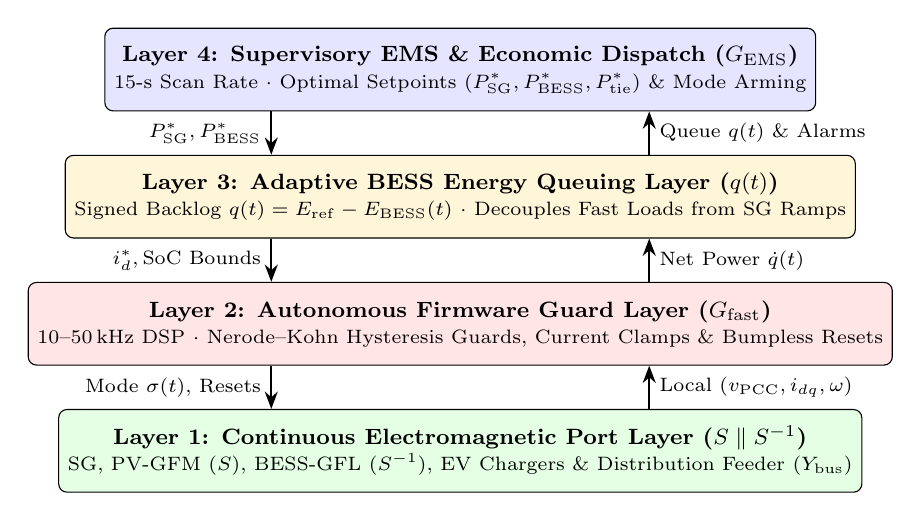
\begin{tikzpicture}[
    node distance=0.55cm,
    layer/.style={draw, rounded corners=3pt, minimum width=8.6cm, minimum height=1.05cm, align=center, font=\footnotesize\bfseries},
    arr/.style={-{Stealth[length=2.2mm]}, thick}
]
\node[layer, fill=blue!10] (L4) {Layer 4: Supervisory EMS \& Economic Dispatch ($G_{\mathrm{EMS}}$) \\ \normalfont\scriptsize 15-s Scan Rate $\cdot$ Optimal Setpoints $(P_{\mathrm{SG}}^*, P_{\mathrm{BESS}}^*, P_{\mathrm{tie}}^*)$ \& Mode Arming};
\node[layer, fill=amber!15, below=of L4] (L3) {Layer 3: Adaptive BESS Energy Queuing Layer ($q(t)$) \\ \normalfont\scriptsize Signed Backlog $q(t) = E_{\mathrm{ref}} - E_{\mathrm{BESS}}(t)$ $\cdot$ Decouples Fast Loads from SG Ramps};
\node[layer, fill=red!10, below=of L3] (L2) {Layer 2: Autonomous Firmware Guard Layer ($G_{\mathrm{fast}}$) \\ \normalfont\scriptsize 10--50\,kHz DSP $\cdot$ Nerode--Kohn Hysteresis Guards, Current Clamps \& Bumpless Resets};
\node[layer, fill=green!10, below=of L2] (L1) {Layer 1: Continuous Electromagnetic Port Layer ($S \parallel S^{-1}$) \\ \normalfont\scriptsize SG, PV-GFM ($S$), BESS-GFL ($S^{-1}$), EV Chargers \& Distribution Feeder ($Y_{\mathrm{bus}}$)};

\draw[arr] ([xshift=-2.4cm]L4.south) -- node[left, font=\scriptsize]{$P_{\mathrm{SG}}^*, P_{\mathrm{BESS}}^*$} ([xshift=-2.4cm]L3.north);
\draw[arr] ([xshift=2.4cm]L3.north) -- node[right, font=\scriptsize]{Queue $q(t)$ \& Alarms} ([xshift=2.4cm]L4.south);

\draw[arr] ([xshift=-2.4cm]L3.south) -- node[left, font=\scriptsize]{$i_d^*, \mathrm{SoC}$ Bounds} ([xshift=-2.4cm]L2.north);
\draw[arr] ([xshift=2.4cm]L2.north) -- node[right, font=\scriptsize]{Net Power $\dot{q}(t)$} ([xshift=2.4cm]L3.south);

\draw[arr] ([xshift=-2.4cm]L2.south) -- node[left, font=\scriptsize]{Mode $\sigma(t)$, Resets} ([xshift=-2.4cm]L1.north);
\draw[arr] ([xshift=2.4cm]L1.north) -- node[right, font=\scriptsize]{Local $(v_{\mathrm{PCC}}, i_{dq}, \omega)$} ([xshift=2.4cm]L2.south);
\end{tikzpicture}%
}
\caption{Four-layer cyber-physical smart microgrid control hierarchy.}
\label{fig:system_stack}
\end{figure}

\section{Physical Parallel Bus vs. Causal Port Architecture}
A common conceptual pitfall in inverter-dominated grids is conflating physical circuit wiring with control signal flow. Electrically, all converters, synchronous machines, loads, and tie-lines connect in \emph{parallel} across the common AC bus ($v_{\mathrm{PCC}}$), as shown in Fig.~\ref{fig:one_line}. No physical switches rewire the bus when a battery reverses power from charging ($P_{\mathrm{BESS}} < 0$) to discharging ($P_{\mathrm{BESS}} > 0$); rather, its active current reference $i_d^* = 2 P_{\mathrm{BESS}}^* / (3 v_d)$ crosses zero continuously.

\begin{figure}[t]
\centering
\resizebox{\columnwidth}{!}{%
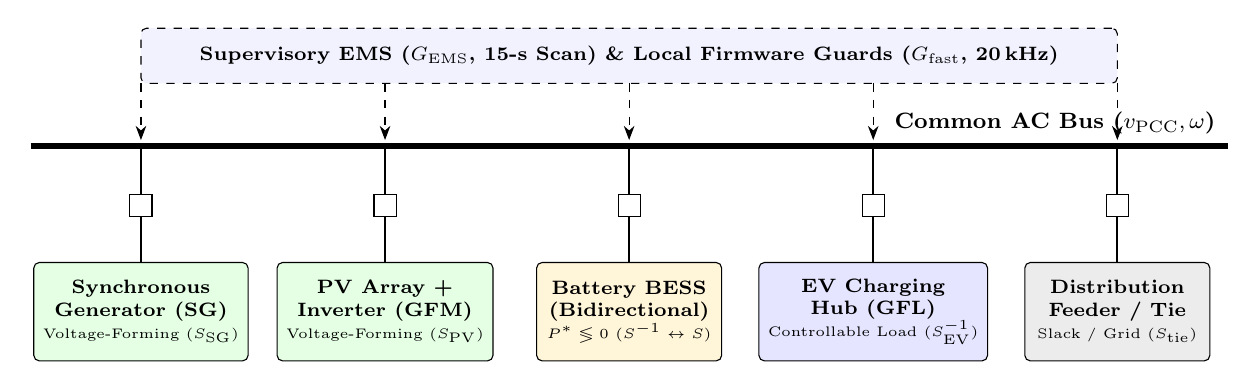
\begin{tikzpicture}[
    dev/.style={draw, rounded corners=2pt, minimum width=2.35cm, minimum height=1.25cm, align=center, font=\scriptsize\bfseries},
    bus/.style={line width=2.2pt},
    wire/.style={thick},
    brk/.style={draw, fill=white, minimum width=0.28cm, minimum height=0.28cm, inner sep=0pt}
]
% Common AC Bus
\draw[bus] (-7.6, 0) -- (7.6, 0) node[above left, font=\footnotesize\bfseries] {Common AC Bus ($v_{\mathrm{PCC}}, \omega$)};

% 5 well-separated columns: -6.2, -3.1, 0.0, 3.1, 6.2
\node[dev, fill=green!10] (sg) at (-6.2, -2.1) {Synchronous\\Generator (SG)\\ \normalfont\tiny Voltage-Forming ($S_{\mathrm{SG}}$)};
\node[dev, fill=green!10] (pv) at (-3.1, -2.1) {PV Array +\\Inverter (GFM)\\ \normalfont\tiny Voltage-Forming ($S_{\mathrm{PV}}$)};
\node[dev, fill=amber!15] (bess) at (0.0, -2.1) {Battery BESS\\(Bidirectional)\\ \normalfont\tiny $P^* \lessgtr 0$ ($S^{-1} \leftrightarrow S$)};
\node[dev, fill=blue!10] (ev) at (3.1, -2.1) {EV Charging\\Hub (GFL)\\ \normalfont\tiny Controllable Load ($S_{\mathrm{EV}}^{-1}$)};
\node[dev, fill=gray!15] (tie) at (6.2, -2.1) {Distribution\\Feeder / Tie\\ \normalfont\tiny Slack / Grid ($S_{\mathrm{tie}}$)};

\foreach \x/\n in {-6.2/sg, -3.1/pv, 0.0/bess, 3.1/ev, 6.2/tie} {
    \draw[wire] (\n.north) -- (\x, 0);
    \node[brk] at (\x, -0.75) {};
}

% Supervisory EMS overhead
\node[draw, dashed, rounded corners=2pt, minimum width=12.4cm, minimum height=0.7cm, fill=blue!5, font=\scriptsize\bfseries] (ems) at (0.0, 1.15) {Supervisory EMS ($G_{\mathrm{EMS}}$, 15-s Scan) \& Local Firmware Guards ($G_{\mathrm{fast}}$, 20\,kHz)};
\foreach \x in {-6.2, -3.1, 0.0, 3.1, 6.2} {
    \draw[dashed, -{Stealth[length=1.8mm]}] (\x, 0.8) -- (\x, 0.08);
}
\end{tikzpicture}%
}
\caption{Physical one-line parallel bus configuration with five non-overlapping DER, load, and feeder branches.}
\label{fig:one_line}
\end{figure}

In the signal-flow domain, however, voltage-forming ($S$) and current-forming ($S^{-1}$) units form a closed \emph{feedback loop} around the bus KCL summation node, as depicted in Fig.~\ref{fig:causal_loop}~\cite{Li2022Duality}. Each reconfigurable inverter embeds both continuous kernels behind an autonomous guard router $G_{\mathrm{fast}}$:
\begin{itemize}
    \item \textbf{Forward Path ($S$):} Takes total bus current $i_{\mathrm{bus}}$ and regulates bus voltage $v_{\mathrm{PCC}}$ via droop and virtual impedance $Z_v$.
    \item \textbf{Feedback Path ($S^{-1}$):} Senses $v_{\mathrm{PCC}}$ via a phase-locked loop (PLL) and injects regulated current $i_{\mathrm{GFL}}$.
\end{itemize}

\begin{figure}[t]
\centering
\resizebox{\columnwidth}{!}{%
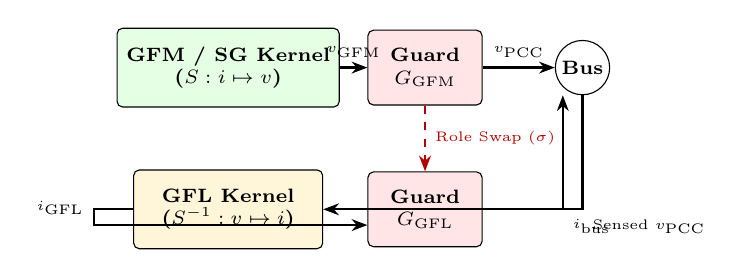
\begin{tikzpicture}[
    blk/.style={draw, rounded corners=2pt, minimum width=2.4cm, minimum height=1.0cm, align=center, font=\scriptsize\bfseries},
    grd/.style={draw, fill=red!10, rounded corners=2pt, minimum width=1.45cm, minimum height=0.95cm, align=center, font=\scriptsize\bfseries},
    arr/.style={-{Stealth[length=2mm]}, thick}
]
\node[blk, fill=green!10] (S) at (-2.4, 0) {GFM / SG Kernel\\($S: i \mapsto v$)};
\node[grd] (G1) at (0.1, 0) {Guard\\$G_{\mathrm{GFM}}$};
\node[circle, draw, inner sep=1.5pt, font=\scriptsize\bfseries] (bus) at (2.1, 0) {Bus};

\node[blk, fill=amber!15] (Sinv) at (-2.4, -1.8) {GFL Kernel\\($S^{-1}: v \mapsto i$)};
\node[grd] (G2) at (0.1, -1.8) {Guard\\$G_{\mathrm{GFL}}$};

\draw[arr] (S.east) -- node[above, font=\tiny]{$v_{\mathrm{GFM}}$} (G1.west);
\draw[arr] (G1.east) -- node[above, font=\tiny]{$v_{\mathrm{PCC}}$} (bus.west);

\draw[arr] (bus.south) |- node[below right, font=\tiny]{Sensed $v_{\mathrm{PCC}}$} (Sinv.east);
\draw[arr] (Sinv.west) -- ++(-0.5,0) |- node[above left, font=\tiny]{$i_{\mathrm{GFL}}$} ([yshift=-0.2cm]G2.west);
\draw[arr] (G2.east) -| node[below right, font=\tiny]{$i_{\mathrm{bus}}$} ([xshift=-0.25cm]bus.south);

\draw[dashed, arr, red!70!black] (G1.south) -- node[right, font=\tiny]{Role Swap ($\sigma$)} (G2.north);
\end{tikzpicture}%
}
\caption{System-level causal feedback loop pairing forward voltage-forming ($S$) and feedback current-forming ($S^{-1}$) operators through autonomous guard routers.}
\label{fig:causal_loop}
\end{figure}

For any connected electrical island of $M$ branches, algebraic solvability of the network DAE requires the \emph{topological well-posedness invariant}:
\begin{equation}
    \sum_{k=1}^{M} \mathbb{I}(\sigma_k = \mathrm{GFM}) + \mathbb{I}(\text{SG/Tie Closed}) \ge 1,
    \label{eq:wellposed}
\end{equation}
ensuring at least one causal voltage source anchors $v_{\mathrm{PCC}}$ at every instant.

\section{Group-Theoretic Symmetries vs. Causal Hybrid Dynamics}
The algebraic structure of the microgrid separates cleanly into invertible group symmetries and causal hybrid restrictions:
\begin{enumerate}
    \item \textbf{Rotational Frame Symmetry ($\mathrm{SO}(2)$):} Transforming three-phase $abc$ variables into rotating $dq$ frames is an action of the circle group $\mathrm{SO}(2)$ parametrized by angle $\theta(t)$, with exact inverse $T(\theta)^{-1} = T(-\theta)$.
    \item \textbf{Port-Duality Involution ($\mathbb{Z}_2$):} Swapping voltage-forming and current-forming roles—i.e., $(v, Z) \leftrightarrow (i, Y)$ or $S \leftrightarrow S^{-1}$—forms an action of the cyclic group $\mathbb{Z}_2 = \{e, \tau\}$ with $\tau^2 = e$~\cite{Li2022Duality}.
    \item \textbf{Role Permutations ($\mathfrak{S}_M$):} Reassigning which subset of $M$ parallel converters acts as voltage-forming masters vs. current-forming followers acts as a permutation on mode vectors $\boldsymbol{\sigma} = (\sigma_1, \dots, \sigma_M)$.
\end{enumerate}

While group elements are unconditionally invertible ($g \cdot g^{-1} = e$), physical realizability breaks symmetry. Dynamic properness (integrators vs. pure differentiators), inverter thermal current limits ($\|i_{dq}\| \le I_{\max}$), and the invariant~\eqref{eq:wellposed} forbid arbitrary group compositions. Furthermore, hysteresis bands and dwell timers $\tau_{\mathrm{dwell}}$ prevent Zeno chattering~\cite{Nerode1993,Simic2005}, restricting transitions to a directed \emph{groupoid / specialization poset} (Fig.~\ref{fig:group_causality}).

\begin{figure}[t]
\centering
\resizebox{\columnwidth}{!}{%
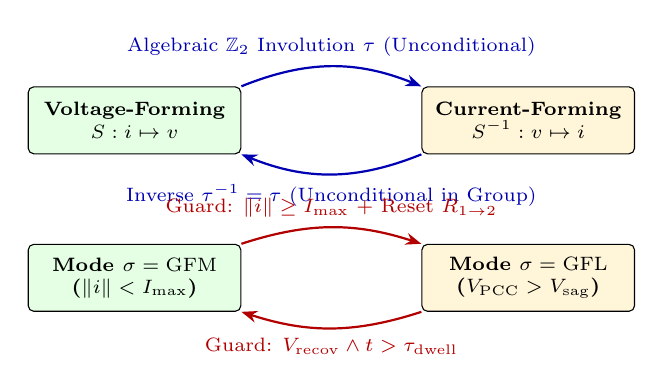
\begin{tikzpicture}[
    st/.style={draw, rounded corners=2pt, minimum width=2.7cm, minimum height=0.85cm, align=center, font=\scriptsize\bfseries},
    arr/.style={-{Stealth[length=2mm]}, thick}
]
\node[st, fill=green!10] (A) at (-2.5, 0) {Voltage-Forming\\$S: i \mapsto v$};
\node[st, fill=amber!15] (B) at (2.5, 0) {Current-Forming\\$S^{-1}: v \mapsto i$};

\draw[arr, bend left=22, blue!70!black] (A.north east) to node[above, font=\scriptsize]{Algebraic $\mathbb{Z}_2$ Involution $\tau$ (Unconditional)} (B.north west);
\draw[arr, bend left=22, blue!70!black] (B.south west) to node[below, font=\scriptsize]{Inverse $\tau^{-1} = \tau$ (Unconditional in Group)} (A.south east);

\node[st, fill=green!10] (A2) at (-2.5, -2.0) {Mode $\sigma = \mathrm{GFM}$\\($\|i\| < I_{\max}$)};
\node[st, fill=amber!15] (B2) at (2.5, -2.0) {Mode $\sigma = \mathrm{GFL}$\\($V_{\mathrm{PCC}} > V_{\mathrm{sag}}$)};

\draw[arr, bend left=18, red!70!black] (A2.north east) to node[above, font=\scriptsize]{Guard: $\|i\| \ge I_{\max}$ + Reset $R_{1\to 2}$} (B2.north west);
\draw[arr, bend left=18, red!70!black] (B2.south west) to node[below, font=\scriptsize]{Guard: $V_{\mathrm{recov}} \wedge t > \tau_{\mathrm{dwell}}$} (A2.south east);
\end{tikzpicture}%
}
\caption{Contrast between unconditional $\mathbb{Z}_2$ algebraic port duality (top) and guard-restricted causal transitions in the hybrid firmware layer (bottom).}
\label{fig:group_causality}
\end{figure}

\section{Adaptive Queuing Layer and Finite Energy Buffers}
From the perspective of bulk synchronous generators constrained by mechanical ramp limits ($|\dot{P}_{\mathrm{SG}}| \le R_{\max}$) and discrete 15-second EMS updates, distributed BESS units form an \emph{Adaptive Queuing Layer}. Unlike data routers that buffer packets by delaying delivery, the BESS serves stochastic EV and PV net load changes instantaneously while accumulating the cumulative energy imbalance in a \emph{signed energy queue}:
\begin{equation}
    q(t) = E_{\mathrm{ref}} - E_{\mathrm{BESS}}(t) = \int_{0}^{t} \big(\lambda(\tau) - \mu(\tau)\big)\,d\tau,
    \label{eq:queue_dyn}
\end{equation}
where $\lambda(t) = P_{\mathrm{EV}}(t) - P_{\mathrm{PV}}(t)$ is the net exogenous power arrival rate and $\mu(t) = P_{\mathrm{SG}}(t) + P_{\mathrm{tie}}(t)$ is the bulk service rate. Positive backlog ($q > 0$) represents an energy deficit requiring upward SG ramping; negative backlog ($q < 0$) represents absorbed surplus energy.

Classical infinite-buffer queuing models yield the asymptotic stability condition $\bar{\lambda} < \bar{\mu}$, which is useful only for nominal reserve sizing. Physically, both computer routers and battery systems possess strictly finite buffers. In our microgrid, the energy queue is bounded by hard state-of-charge walls and inverter power bandwidth limits:
\begin{equation}
    q_{\min} \le q(t) \le q_{\max}, \qquad |\dot{q}(t)| = |P_{\mathrm{BESS}}(t)| \le P_{\max}.
    \label{eq:queue_bounds}
\end{equation}
Using deterministic Network Calculus~\cite{LeBoudec2001}, if net load arrivals satisfy a $(\sigma_a, \rho_a)$ affine envelope and bulk SG generation provides a rate-latency service curve $\beta(t) = R_{\mathrm{svc}}[t - T_{\mathrm{EMS}}]^+$ (accounting for the 15-second EMS scan latency $T_{\mathrm{EMS}}$), the worst-case energy queue excursion is bounded by $\Delta q_{\max} \le \sigma_a + \rho_a T_{\mathrm{EMS}}$. Whenever stochastic bursts exceed $\Delta q_{\max}$ and drive $q(t)$ onto the buffer walls, $G_{\mathrm{fast}}$ enforces non-linear boundary actions summarized in Table~\ref{tab:guards}.

\begin{table}[t]
\centering
\caption{Hierarchical Guard Actions Across Buffer \& Port Boundaries}
\label{tab:guards}
\begin{tabular}{@{}p{2.1cm}p{2.5cm}p{3.2cm}@{}}
\toprule
\textbf{Boundary Condition} & \textbf{Active Layer} & \textbf{Causal / Hybrid Action} \\
\midrule
$\|i_{\mathrm{PV}}\| \ge I_{\max}$ & $G_{\mathrm{fast}}$ (Firmware) & PV swaps $\mathrm{GFM} \to \mathrm{GFL}_{\mathrm{clamp}}$ ($S \to S^{-1}$). \\
$V_{\mathrm{PCC}} \le V_{\mathrm{sag}}$ & $G_{\mathrm{fast}}$ (Firmware) & BESS swaps $\mathrm{GFL} \to \mathrm{GFM}$ ($S^{-1} \to S$) with bumpless angle reset. \\
$q(t) \ge q_{\max}$ & $G_{\mathrm{fast}}$ (Queue Wall) & EV charging throttled by 50\% until SG drains backlog. \\
$q(t) \le q_{\min}$ & $G_{\mathrm{fast}}$ (Queue Floor) & PV frequency-watt curtailment shifts off MPPT. \\
$t = k \cdot 15\,\mathrm{s}$ & $G_{\mathrm{EMS}}$ (Supervisory) & Updates $P_{\mathrm{SG}}^*$ proportional to $q(t)$ and restores $V_{\mathrm{PCC}} \to 1.0\,\mathrm{pu}$. \\
\bottomrule
\end{tabular}
\end{table}

\section{Configuration Workflow and EMT Implementation}
To deploy this architecture in Electromagnetic Transient (EMT) studies (such as `PowerSimulationsDynamics.jl`~\cite{Lara2024PSID} or custom DAE solvers), engineers follow a four-step workflow:
\begin{enumerate}
    \item \textbf{Baseline Causality Assignment:} Assign voltage-forming ($S$) status to the primary GFM/SG anchor and current-forming ($S^{-1}$) status to bidirectional BESS and EV rectifiers, satisfying~\eqref{eq:wellposed}.
    \item \textbf{Signed Power Dispatch Setup:} Configure BESS outer loops to accept signed setpoints $P_{\mathrm{BESS}}^* \in [-P_{\max}, +P_{\max}]$ with smooth zero-crossing current references.
    \item \textbf{Staggered Firmware Guard Tuning:} Tune $G_{\mathrm{fast}}$ thresholds in `DiscreteCallback` routines so overcurrent clamps fire faster ($<1\,\mathrm{ms}$) than undervoltage GFM takeovers ($5\text{--}10\,\mathrm{ms}$), with hysteresis margins preventing Zeno chattering.
    \item \textbf{Supervisory 15-s Queue Loop:} Implement $G_{\mathrm{EMS}}$ via `PeriodicCallback` at $15\,\mathrm{s}$ intervals to drive SG mechanical power references from the energy queue state $q(t)$.
\end{enumerate}

\section{Simulation Case Study}
To validate the four-layer hierarchy, a 60-second EMT simulation was executed in Julia using `DifferentialEquations.jl` and `DiffEqCallbacks.jl`. Initially ($t = 0\text{--}20\,\mathrm{s}$), PV-GFM generates $0.60\,\mathrm{pu}$, EV load draws $0.20\,\mathrm{pu}$, and BESS charges at $P_{\mathrm{BESS}}^* = -0.40\,\mathrm{pu}$ ($V_{\mathrm{PCC}} = 1.00\,\mathrm{pu}$). At $t = 20\,\mathrm{s}$, a heavy EV charging surge ($P_{\mathrm{EV}} \to 1.15\,\mathrm{pu}$) pushes PV-GFM past its $1.45\,\mathrm{pu}$ current ceiling, triggering an immediate firmware switch to $\mathrm{GFL}_{\mathrm{clamp}}$ ($S \to S^{-1}$). Within $40\,\mathrm{ms}$ ($t = 20.04\,\mathrm{s}$), bus voltage sags to $0.917\,\mathrm{pu}$ and BESS autonomously takes over as GFM ($S^{-1} \to S$), arresting the voltage drop. As BESS discharges to serve the EV surge while SG waits for the next EMS scan, $q(t)$ climbs until hitting $q_{\max} = 4.0\,\mathrm{pu\cdot s}$ at $t = 41.44\,\mathrm{s}$, triggering autonomous EV charge throttling. At $t = 45\,\mathrm{s}$, $G_{\mathrm{EMS}}$ commands $P_{\mathrm{SG}}^* = 0.842\,\mathrm{pu}$, draining $q(t)$ and restoring $V_{\mathrm{PCC}}$ to $1.003\,\mathrm{pu}$ (Fig.~\ref{fig:sim_results}).

\begin{figure}[t]
\centering
\resizebox{\columnwidth}{!}{%
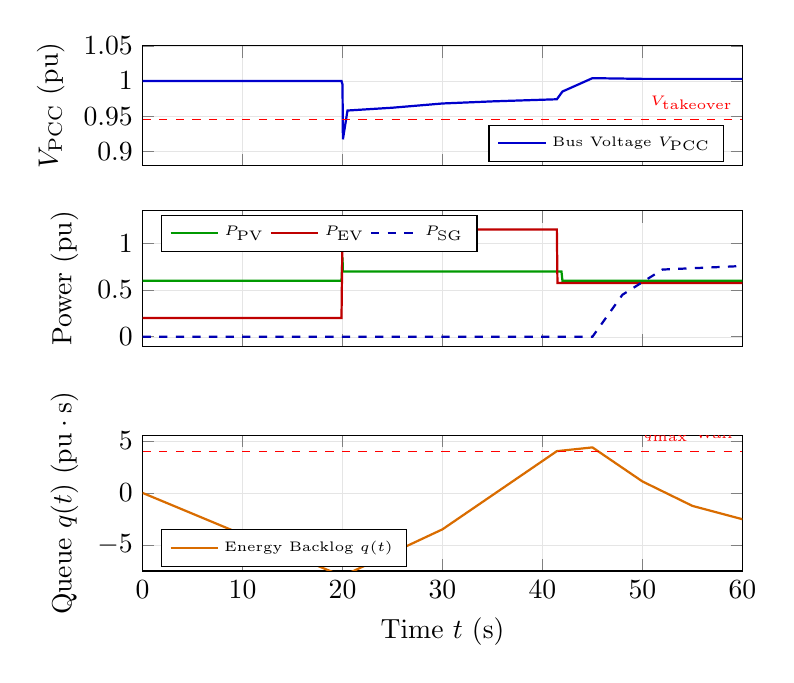
\begin{tikzpicture}
\begin{axis}[
    name=ax1,
    width=9.2cm, height=3.1cm,
    xmin=0, xmax=60, ymin=0.88, ymax=1.05,
    ylabel={$V_{\mathrm{PCC}}$ (pu)},
    xticklabels=\empty,
    grid=both, grid style={line width=.1pt, draw=gray!20},
    legend pos=south east, legend style={font=\tiny}
]
\addplot[thick, blue!80!black] table[row sep=crcr] {
t v \\
0.0 1.000 \\ 10.0 1.000 \\ 19.9 1.000 \\ 20.0 0.995 \\ 20.04 0.917 \\ 20.5 0.958 \\ 25.0 0.962 \\ 30.0 0.968 \\ 35.0 0.971 \\ 41.44 0.974 \\ 42.0 0.985 \\ 45.0 1.004 \\ 50.0 1.003 \\ 60.0 1.003 \\
};
\addlegendentry{Bus Voltage $V_{\mathrm{PCC}}$}
\draw[dashed, red] (axis cs:0,0.945) -- (axis cs:60,0.945) node[above left, font=\tiny, red]{$V_{\mathrm{takeover}}$};
\end{axis}

\begin{axis}[
    name=ax2,
    at={(ax1.below south west)}, anchor=above north west, yshift=-0.22cm,
    width=9.2cm, height=3.3cm,
    xmin=0, xmax=60, ymin=-0.1, ymax=1.35,
    ylabel={Power (pu)},
    xticklabels=\empty,
    grid=both, grid style={line width=.1pt, draw=gray!20},
    legend pos=north west, legend style={font=\tiny, legend columns=3}
]
\addplot[thick, green!60!black] table[row sep=crcr] {
t p \\
0.0 0.60 \\ 19.9 0.60 \\ 20.0 0.85 \\ 20.04 0.70 \\ 41.9 0.70 \\ 42.0 0.60 \\ 60.0 0.60 \\
};
\addlegendentry{$P_{\mathrm{PV}}$}
\addplot[thick, red!75!black] table[row sep=crcr] {
t p \\
0.0 0.20 \\ 19.9 0.20 \\ 20.0 1.15 \\ 41.44 1.15 \\ 41.5 0.575 \\ 60.0 0.575 \\
};
\addlegendentry{$P_{\mathrm{EV}}$}
\addplot[thick, blue!70!black, dashed] table[row sep=crcr] {
t p \\
0.0 0.00 \\ 30.0 0.00 \\ 45.0 0.00 \\ 48.0 0.45 \\ 52.0 0.72 \\ 60.0 0.758 \\
};
\addlegendentry{$P_{\mathrm{SG}}$}
\end{axis}

\begin{axis}[
    name=ax3,
    at={(ax2.below south west)}, anchor=above north west, yshift=-0.22cm,
    width=9.2cm, height=3.3cm,
    xmin=0, xmax=60, ymin=-7.5, ymax=5.5,
    xlabel={Time $t$ (s)},
    ylabel={Queue $q(t)$ ($\mathrm{pu\cdot s}$)},
    grid=both, grid style={line width=.1pt, draw=gray!20},
    legend pos=south west, legend style={font=\tiny}
]
\addplot[thick, orange!85!black] table[row sep=crcr] {
t q \\
0.0 0.00 \\ 15.0 -6.00 \\ 20.0 -8.00 \\ 30.0 -3.50 \\ 41.44 4.01 \\ 45.0 4.37 \\ 50.0 1.10 \\ 55.0 -1.25 \\ 60.0 -2.53 \\
};
\addlegendentry{Energy Backlog $q(t)$}
\draw[dashed, red] (axis cs:0,4.0) -- (axis cs:60,4.0) node[above left, font=\tiny, red]{$q_{\max}$ Wall};
\end{axis}
\end{tikzpicture}%
}
\caption{60-second hybrid EMT simulation showing the $t = 20\,\mathrm{s}$ causal role reversal ($S \leftrightarrow S^{-1}$), $q_{\max}$ EV throttling guard, and 15-s EMS SG ramp drainage.}
\label{fig:sim_results}
\end{figure}

\section*{Acknowledgment}
The author acknowledges Google Gemini for assistance with mathematical formalization, TikZ/PGFPlots diagram generation, Julia simulation structuring, and editorial refinement.

\begin{thebibliography}{1}
\bibitem{Li2022Duality}
Y.~Li, Y.~Gu, and T.~C.~Green, ``Revisiting grid-forming and grid-following inverters: A duality theory,'' \emph{IEEE Trans. Power Syst.}, vol.~37, no.~6, pp.~4541--4554, Nov.~2022.

\bibitem{Mesarovic1970}
M.~D.~Mesarovi\'{c}, D.~Macko, and Y.~Takahara, \emph{Theory of Hierarchical, Multilevel, Systems}. New York, NY, USA: Academic Press, 1970.

\bibitem{Nerode1993}
A.~Nerode and W.~Kohn, ``Models for hybrid systems: Automata, topologies, controllability, observability,'' in \emph{Hybrid Systems}, ser. Lecture Notes in Computer Science, vol.~736. Berlin, Germany: Springer, 1993, pp.~317--356.

\bibitem{Simic2005}
S.~N.~Simi\'{c}, K.~H.~Johansson, J.~Lygeros, and S.~Sastry, ``Towards a geometric theory of hybrid systems,'' \emph{Dyn. Continuous, Discrete Impulsive Syst., Ser. B}, vol.~12, no.~5--6, pp.~649--687, 2005.

\bibitem{LeBoudec2001}
J.-Y.~Le~Boudec and P.~Thiran, \emph{Network Calculus: A Theory of Deterministic Queuing Systems for the Internet}. Berlin, Germany: Springer, 2001.

\bibitem{Gelenbe2015}
E.~Gelenbe and E.~T.~Ceran, ``Energy packet networks with energy harvesting,'' \emph{IEEE Access}, vol.~4, pp.~1321--1331, 2016.

\bibitem{Lara2024PSID}
J.~D.~Lara, R.~Henriquez-Auba, D.~Ramasubramanian, S.~Dhople, C.~Barrows, and D.~S.~Callaway, ``PowerSimulationsDynamics.jl---An open-source modeling package for modern power systems with inverter-based resources,'' \emph{SoftwareX}, vol.~26, 2024, Art.~no.~101668.
\end{thebibliography}

\end{document}
